
In the past years, the study of the VBS processes has attracted lots of interests from the theory community, (see {\emph e.g.} the review~\cite{Rauch:2016pai}).
The acivities range from providing precise predictions for the VBS signal and background processes in the Standard Model, to studying the sensitivity of these 
processes on new physics effects, by mean of effective theories or by studying the polarisation patterns of the heavy gauge bosons involved.
The program of the meeting reflects these avenues.

\subsection{Complete NLO corrections to ${\rm W^+ W^+}$ scattering - M. Pellen}

The first VBS process that has been observed during the run~I of the LHC is the same-sign WW production~\cite{Aad:2014zda,Aaboud:2016ffv,Khachatryan:2014sta}.
This observation has already been confirmed by a measurement of the CMS collaboration at the 13 TeV run~II~\cite{CMS:2017adb}.
In view of the growing mole of data which will be collected by the experiments, and of the consequent reduction of the uncertainties affecting these measurements, precise theoretical predictions become necessary.

In that respect NLO QCD and EW corrections to such signature should be computed.
So far, NLO have focused on NLO QCD corrections to the VBS process~\cite{Jager:2009xx,Jager:2011ms,Denner:2012dz,Rauch:2016pai} and its QCD-induced irreducible background process~\cite{Melia:2010bm,Melia:2011gk,Campanario:2013gea,Baglio:2014uba,Rauch:2016pai}.
No NLO EW have been computed and the NLO QCD corrections relied on the so-called VBS approximation.
In Refs.~\cite{Biedermann:2016yds,Biedermann:2017bss}, for the first, all leading order (LO) and next-to-leading (NLO) contributions to the full ${\rm p}{\rm p}\to\mu^+\nu_\mu{\rm e}^+\nu_{\rm e}{\rm j}{\rm j}$ process have been reported.
As the full amplitudes are used, this amounts to compute three LO contributions and four NLO contributions.
At LO, the three contributions are the EW process (order $\mathcal{O}{\left(\alpha^{6}\right)}$), its QCD-induced counterpart (order $\mathcal{O}{\left(\alpha_{\rm s}\alpha^{5}\right)}$) as well as the interference (order $\mathcal{O}{\left(\alpha_{\rm s}^2\alpha^{4}\right)}$).
Due to the VBS event selection applied to the final state, the full process is dominated by the purely EW contribution (see Table~\ref{table:LOVBS}).
This EW contribution feature the VBS diagrams but also background diagrams where for example the W bosons are simply radiated from the quark lines.

\begin{table}
\begin{center}
\begin{tabular}{|l||c|c|c||c|}
\hline
Order & $\mathcal{O}{\left(\alpha^{6}\right)}$ & $\mathcal{O}{\left(\alpha_{\rm s}\alpha^{5}\right)}$ & $\mathcal{O}{\left(\alpha_{\rm s}^2\alpha^{4}\right)}$ & Sum \\
\hline
\hline
${\sigma_{\mathrm{LO}}}$ [fb] 
& $1.4178(2)$
& $0.04815(2)$
& $0.17229(5)$
& $1.6383(2)$ \\
\hline
\end{tabular}
\end{center}
\caption{
Fiducial cross section~\cite{Biedermann:2017bss} at LO for the process ${\rm p}{\rm p}\to\mu^+\nu_\mu{\rm e}^+\nu_{\rm e}{\rm j}{\rm j}$, at
orders  $\mathcal{O}{\left(\alpha^{6}\right)}$, $\mathcal{O}{\left(\alpha_{\rm s}\alpha^{5}\right)}$, and $\mathcal{O}{\left(\alpha_{\rm s}^2\alpha^{4}\right)}$.
The sum of all the LO contributions is in the last column and all contributions expressed in femtobarn. 
The statistical uncertainty from the Monte Carlo integration on the last digit is given in parenthesis.}
\label{table:LOVBS}
\end{table}

At NLO, the four contributions arise at the orders $\mathcal{O}{\left(\alpha^{7}\right)}$, $\mathcal{O}{\left(\alpha_{\rm s}\alpha^{6}\right)}$, $\mathcal{O}{\left(\alpha_{\rm s}^{2}\alpha^{5}\right)}$, and $\mathcal{O}{\left(\alpha_{\rm s}^{3}\alpha^{4}\right)}$. 
An interesting feature is that the orders $\mathcal{O}{\left(\alpha_{\rm s}\alpha^{6}\right)}$ and $\mathcal{O}{\left(\alpha_{\rm s}^{2}\alpha^{5}\right)}$ receive both EW and QCD corrections.
Thus, at NLO (as opposed to LO) it is not possible to strictly distinguish the EW process from the QCD-induced process.
As it can be seen from Table~\ref{table:NLOVBS}, at the level of the fiducial cross section, the largest corrections are the one of order $\mathcal{O}{\left(\alpha^{7}\right)}$.
These are the NLO EW corrections to the EW processes.

\begin{table}
\begin{center}
\begin{tabular}{|l||c|c|c|c||c|}
\hline
Order & $\mathcal{O}{\left(\alpha^{7}\right)}$ & $\mathcal{O}{\left(\alpha_{\rm s}\alpha^{6}\right)}$ & $\mathcal{O}{\left(\alpha_{\rm s}^{2}\alpha^{5}\right)}$ & $\mathcal{O}{\left(\alpha_{\rm s}^{3}\alpha^{4}\right)}$ & Sum \\
\hline
\hline 
${\delta \sigma_{\mathrm{NLO}}}$ [fb] 
& $-0.2169(3)$ 
& $-0.0568(5)$
& $-0.00032(13)$
& $-0.0063(4)$ 
& $-0.2804(7)$ \\
\hline
$\delta \sigma_{\mathrm{NLO}}/\sigma_{\rm LO}$ [\%] & $-13.2$ & $-3.5$ & $0.0$ & $-0.4$ & $-17.1$ \\
\hline
\end{tabular}
\end{center}
\caption{
NLO corrections~\cite{Biedermann:2017bss} for the process ${\rm p}{\rm p}\to\mu^+\nu_\mu{\rm e}^+\nu_{\rm e}{\rm j}{\rm j}$ at the orders 
$\mathcal{O}{\left(\alpha^{7}\right)}$, $\mathcal{O}{\left(\alpha_{\rm s}\alpha^{6}\right)}$, $\mathcal{O}{\left(\alpha_{\rm s}^{2}\alpha^{5}\right)}$, and $\mathcal{O}{\left(\alpha_{\rm s}^{3}\alpha^{4}\right)}$.
The sum of all the NLO contributions is in the last column.
The contribution $\delta\sigma_{\mathrm{NLO}}$ corresponds to the absolute correction while $\delta \sigma_{\mathrm{NLO}}/\sigma_{\rm LO}$ gives the relative correction normalised to the sum of all LO contributions.
The absolute contributions are expressed in femtobarn while the relative ones are expressed in per cent.
The statistical uncertainty from the Monte Carlo integration on the last digit is given in parenthesis.}
\label{table:NLOVBS}
\end{table}

All these different contributions can also be seen in two differential distributions in the the transverse momentum for the hardest jet and invariant mass for the two leading jets in Fig.~\ref{fig:VBSALL}.
Each contribution (both LO and NLO) shows distinctive features.
At LO, the QCD induced process as well as the interference are rather suppressed due to the typical VBS event selection (as for the fiducial cross section).
This is exemplified in the invariant mass of the two leading jet where at high invariant mass, the QCD-induced background becomes negligible.
At NLO, the bulk of the corrections originate from the large EW to the EW process at order $\mathcal{O}{\left(\alpha^{7}\right)}$.
In particular they display the typical behaviour of Sudakov logarithms that grow large in the high energy limit.
Note that the contribution from initial state photon is also shown but is not taken into account in the definition of the NLO predictions.
This contribution is rather small and fairly constant in shape over the whole range studied here.
Finally, as at NLO, in it is not possible to isolate the EW production from its irreducible backgrounds, a global measurement of the process full ${\rm p}{\rm p}\to\mu^+\nu_\mu{\rm e}^+\nu_{\rm e}{\rm j}{\rm j}$ with all component is desirable.
Hence in Fig.~\ref{fig:VBSAAL_sum}, the sum all the contributions at both LO and NLO is shown in a combined prediction.

\begin{figure}
% \hspace{-2cm}
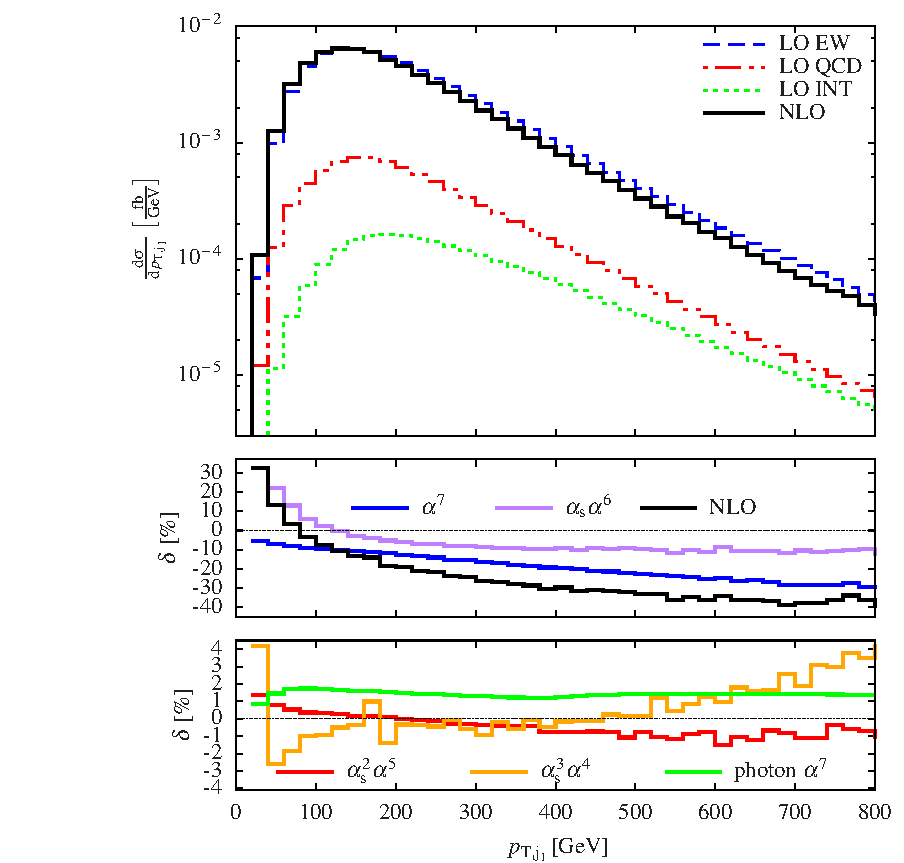
\includegraphics[width=.47\textwidth]{WG1_plots/histogram_transverse_momentum_j1}
\hfill
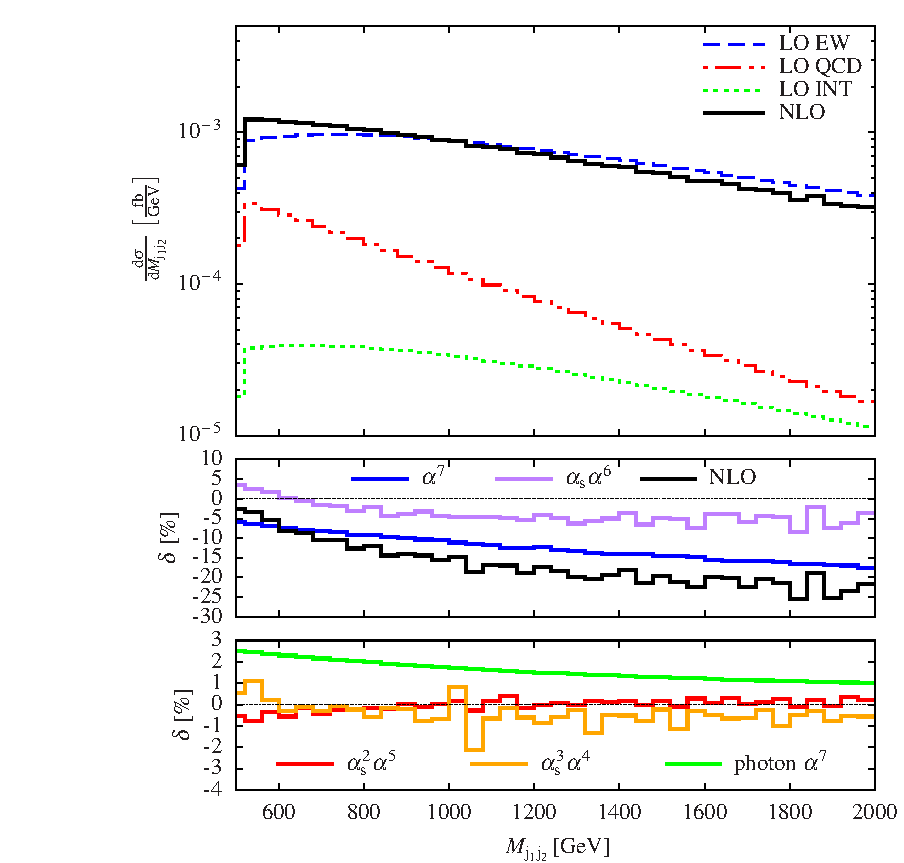
\includegraphics[width=.47\textwidth]{WG1_plots/histogram_invariant_mass_mjj12}
% \vspace*{-1em}
\caption{Differential distributions~\cite{Biedermann:2017bss} for ${\rm p}{\rm p}\to\mu^+\nu_\mu{\rm e}^+\nu_{\rm e}{\rm j}{\rm j}$:
transverse momentum for the hardest jet~(left) and invariant mass for the two leading jets~(right).
The two lower panels show the relative NLO corrections with respect to the full LO in per cent,
defined as $\delta_i = \delta \sigma_{i} / \sum \sigma_{\text{LO}}$, 
where $i=\mathcal{O}{\left(\alpha^{7}\right)},\mathcal{O}{\left(\alpha_{\rm s}\alpha^{6}\right)},\mathcal{O}{\left(\alpha_{\rm s}^2\alpha^{5}\right)},\mathcal{O}{\left(\alpha_{\rm s}^3\alpha^{4}\right)}$.
In addition, the NLO photon-induced contributions of order $\mathcal{O}{\left(\alpha^{7}\right)}$ is provided separately.}
\label{fig:VBSALL}
\end{figure}

\begin{figure}
% \hspace{-2cm}
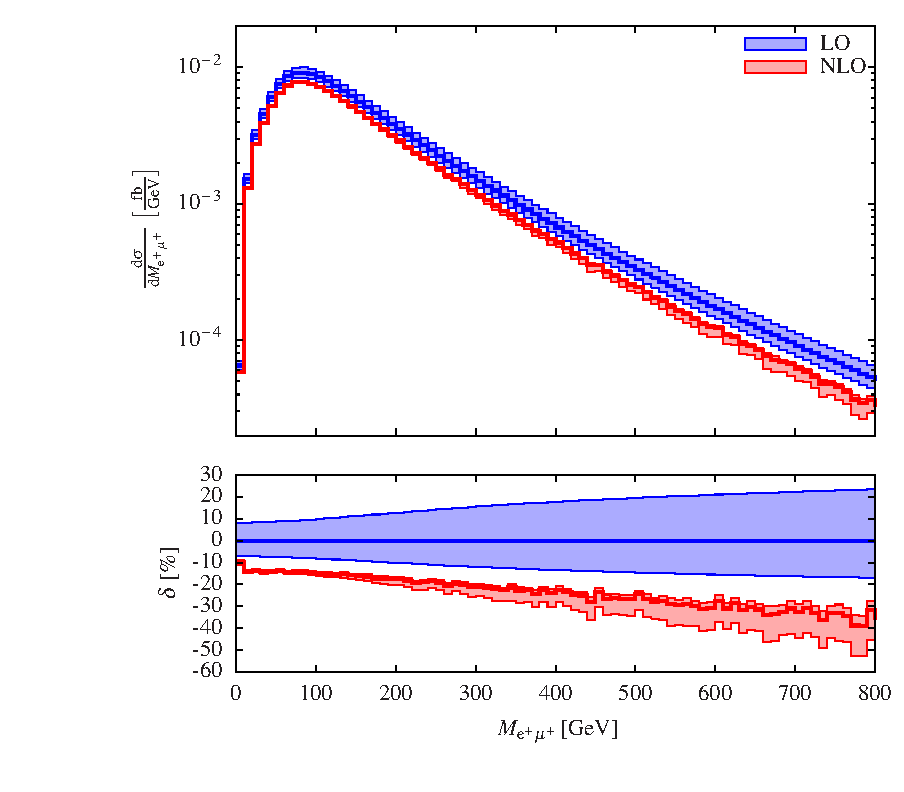
\includegraphics[width=.47\textwidth]{WG1_plots/histogram_invariant_mass_epmu_scale}
\hfill
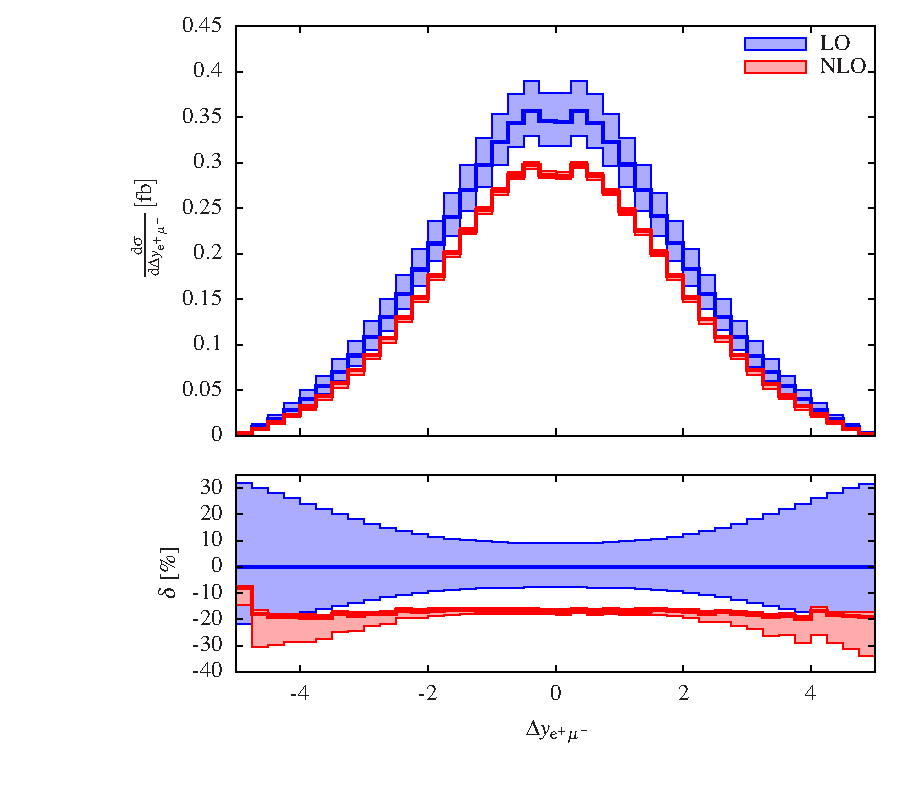
\includegraphics[width=.47\textwidth]{WG1_plots/histogram_rapidity_separation_pomu_scale}
% \vspace*{-1em}
\caption{Differential distributions~\cite{Biedermann:2017bss} for ${\rm p}{\rm p}\to\mu^+\nu_\mu{\rm e}^+\nu_{\rm e}{\rm j}{\rm j}$:
invariant mass of the positron and anti-muon system~(left) and rapidity separation between the electron and anti-muon~(right).
The upper panels show the sum of all LO and NLO contributions with scale variation.
The lower panels show the relative corrections in per cent.}
\label{fig:VBSAAL_sum}
\end{figure}

As shown previously, the EW corrections of order $\mathcal{O}\left(\alpha^7\right)$ are the dominant NLO contributions.
These originate from Sudakov logarithms that grow negatively large in the high energy limit.
This is shown in the differential distribution in the transverse momentum of the hardest jet on the left hand-side of Fig.~\ref{fig:VBSEW}.
Usually these EW corrections are particularly large only in phase space regions which are suppressed.
Hence the impact at the level of the total fiducial cross section is usually rather limited.
This is not the case here where the corrections are already large at the level of the cross section and reach $-16\%$ \cite{Biedermann:2016yds}.
The origin of these large EW corrections are indeed virtual corrections and in particular the ones corresponding to the insertion of massive particles in the scattering process \cite{Biedermann:2016yds}.
Hence, large NLO EW corrections are an intrinsic feature of VBS at the LHC.
As the EW corrections are particularly large, it might be possible to measure them at a high luminosity LHC, hence probing the EW sector of the Standard Model to very high precision.
This is illustrated on the left hand-side of Fig.~\ref{fig:VBSEW} where the band represent the estimated statistical error for a high-luminosity LHC collecting $3000{\rm fb}^{-1}$.

\begin{figure}
% \hspace{-2cm}
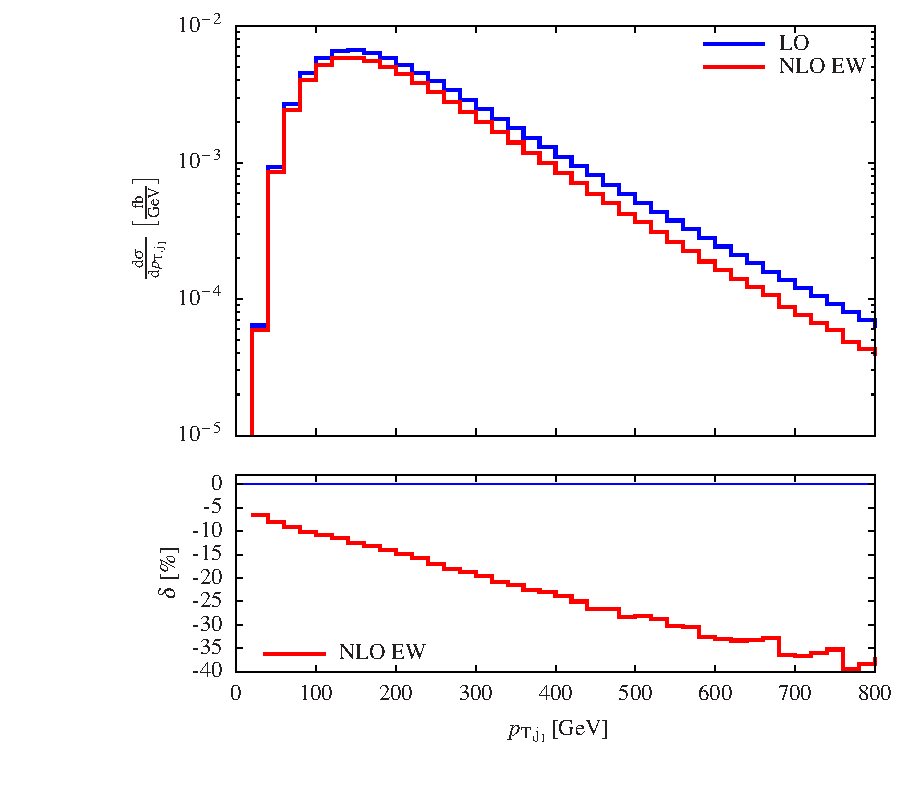
\includegraphics[width=.47\textwidth]{WG1_plots/histogram_transverse_momentum_j1_ew}
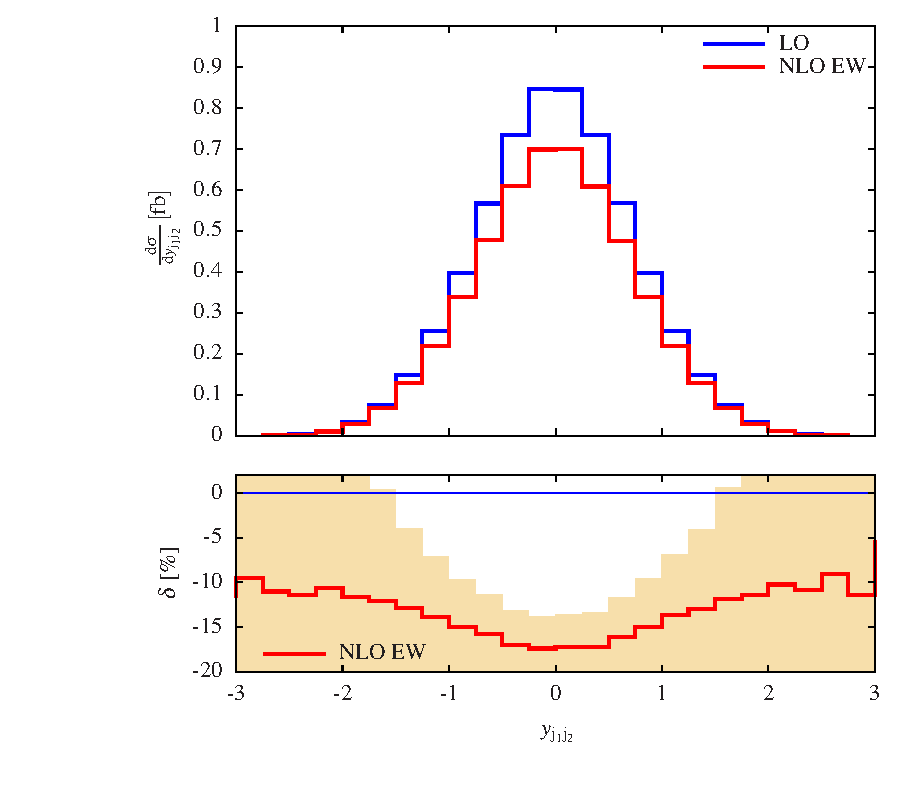
\includegraphics[width=.47\textwidth]{WG1_plots/histogram_rapidity_j1j2_ew}
% \vspace*{-1em}
\caption{Differential distributions~\cite{Biedermann:2016yds} for ${\rm p}{\rm p}\to\mu^+\nu_\mu{\rm e}^+\nu_{\rm e}{\rm j}{\rm j}$ including NLO EW corrections (upper panel) and relative NLO EW corrections (lower panel).
Left plot: Invariant-mass distribution of the four leptons.
Right plot: Rapidity distribution of the leading jet pair.
The yellow band describes the expected statistical experimental uncertainty for a high-luminosity LHC collecting $3000{\rm fb}^{-1}$ and represents a relative variation of $\pm 1/\sqrt{N_{\rm obs}}$ where $N_{\rm obs}$ is the number of observed events in each bin.}
\label{fig:VBSEW}
\end{figure}

\subsection{Monte Carlo comparisons for ${\rm W^+ W^+}$ scattering - M. Zaro}
In the last decade many codes capable of performing VBS simulations have appeared; within a network such as VBSCan, it is therefore natural to perform 
a quantitative comparison of these codes, both to cross-validate the results and to assess the impact of the different approximations which are performed in each tool. In fact, 
already at the LO, when the process ${\rm p}{\rm p}\to\mu^+\nu_\mu{\rm e}^+\nu_{\rm e}{\rm j}{\rm j}$ at $\mathcal O (\alpha^6)$ is considered, the various implementations of VBS differ, for example
by the (non-)inclusion of diagrams with vector bosons in the $s$-channel or by the treatment of interferences between diagrams; the reason of these differences is that, 
when typical signal cuts for VBS are imposed, these effects turn to be totally negligible on rates and distributions.

In our comparison, we use the following codes: {\bf ADD/CHECK CITES} 
{\sc Bonsay}~\cite,
{\sc MadGraph5\_aMC@NLO}~\cite{Alwall:2014hca}, 
{\sc Powheg}~\cite{},
{\sc Recola+MoCaNLO}~\cite{Actis:2012qn,Actis:2016mpe,MoCaNLO}\footnote{To numerically evaluate the one-loop scalar and tensor integrals, {\sc Recola} relies on the {\sc Collier} library \cite{Denner:2014gla,Denner:2016kdg}},
{\sc VBFNLO}~\cite{Arnold:2008rz, Arnold:2011wj, Baglio:2014uba}.
The complete comparison of the codes will be published in a separate work. Here, we present some preliminary results obtained at LO ($\mathcal O (\alpha^6)$) and including
NLO QCD corrections at fixed-order ($\mathcal O (\alpha^6\alpha_s)$, for the process ${\rm p}{\rm p}\to\mu^+\nu_\mu{\rm e}^+\nu_{\rm e}{\rm j}{\rm j}$. In 
Tab.~\ref{tab:wg1_codes} we report on the details of the various codes. In particular, we check whether
\begin{itemize}
    \item all $s-$ and $t/u-$channel diagrams that lead to the considered final state are included;
    \item interferences between diagrams are included at LO;
    \item off-shell contributions and diagrams which do not feature two resonant vector bosons are included;
    \item the so-called ``non-factorizable'' (NF) QCD corrections, that is those corrections where (real or virtual) gluons are exchanged between different quark lines,
        are included;
    \item EW corrections to the $\mathcal O (\alpha^5\alpha_s)$ interference are included. These corrections are of the same order as the NLO QCD corrections to
        the  $\mathcal O (\alpha^6$ term.
\end{itemize}
%
\begin{table}
    \footnotesize
    \begin{tabularx}{\textwidth}{c|c|X|X|X|X|X}
        Contact person  &  Code  &  $\mathcal O(\alpha^6)$ $|s|^2/$ $|t|^2/|u|^2$  &  $\mathcal O(\alpha^6)$ interf.  &  Off-shell  &  NF QCD  &  EW corr. to $\mathcal O(\alpha^5\alpha_s)$  \\
        \hline
        \hline
        A. Karlberg  &  {\sc POWHEG}  &  $t/u$  &  No  &  Yes  &  No  &  No  \\
        M. Pellen    &  {\sc Recola}  &  Yes  &  Yes  &  Yes  &  Yes  &  Yes  \\
        M. Rauch     &  {\sc VBFNLO}  &  Yes  &  No  &  Yes  &  No  &  No  \\
        C. Schwan    &  {\sc BONSAY}  &  $t/u$  &  No  &  Yes, virt. No  &  No  &  No  \\
        M. Zaro      &  {\sc MG5\_aMC}  &  Yes  &  Yes  &  No virt.  &  No  &  No
    \end{tabularx}
    \caption{\label{tab:wg1_codes} Summary of the different properties of the codes employed in the comparison.}
\end{table}
%
INPUT AND SETUP\\
VBS CUTS\\
PLOTS\\
The results of our comparison show an excellent agreement of the different tools at LO, which justify the approximations made in some of these tools not to include certain 
contributions. At NLO, slightly larger (but still below $10\%$) effects can be noticed for example at low dijet invariant mass, where $s-$ channels and interferences are not
as much suppressed as at LO, because of real QCD radiation.


We conclude this session by recalling that the results presented must be regarded as preliminary.
In the coming months, this work will be enlarged to include comparison of predictions at NLO QCD matched to parton shower or with EW corrections, 
as well as to study the effect of changing 
the VBS cuts. The QCD-induced background will also be studied.

\subsection{Polarisation of vector bosons - E. Maina}

It has been argued that new physics model could lead to large contributions to the longitudinal polarisation of heavy gauge bosons [citation?].
Hence it is of prime importance to study the polarisation of the heavy gauge bosons and their effects both in the Standard Model and beyond.
In particular, it is very important to devise methods that allow for such studies.
Thus, a starting point is to establish these methods first for the Standard Model.
In this respect, a new method has been proposed and applied to the scattering of two W bosons of opposite charge.

First, a matrix element squared can be written in a general manner as

\begin{equation}
\label{eq:polarisation}
 \mathcal{A}^2 = \sum_{\lambda} \mathcal{A}^2_{\lambda, \lambda} + \sum_{\lambda \neq \lambda'} \mathcal{A}^2_{\lambda, \lambda'}, 
\end{equation}
%
where $\lambda$ represents the polarisation of the heavy gauge bosons.
Usually the last term of Eq.~\eqref{eq:polarisation} is assumed to be zero.
But this is only true when ones integrates over the full phase space over the variable $\phi$.
In experiments, it is never the case as experimental measurements are never done fully inclusively.
Indeed they always include event selections that cut into the phase space and make the use of a full computation necessary.

Second, an amplitude can be divided into resonant and non-resonant contributions as

\begin{equation}
\mathcal{A} = \mathcal{A}_{\rm res} + \mathcal{A}_{\rm non-res} .
\end{equation}
%
But non-resonant propagators cannot be interpreted as W production.
Hence, one should only retain the resonant part of the process.
To achieve this in a gauge invariant way, one can use the double-pole approximation where only diagrams featuring a two W boson propagator are selected.
This sub-set of diagrams is then evaluation with an on-shell kinematic.
But on-shell kinematics are not unique so one should use an on-shell projection that should fulfil the following criteria:
[To be added]
In such a way, one can set a given polarisation to the W bosons in a gauge invariant manner.

Moving on to the results.
In order to be able to integrate fully over the variable $\phi$, one should consider a typical VBS event selection but without any cuts on the final state leptons.
If one consider a ${\rm W^-}$ polarised and a ${\rm W^-}$ non-polarised, one observes that the effect of the interferences between different polarisations (second term of Eq.~\eqref{eq:polarisation}) is below one per cent at the level of the total cross section.
At the level of differential distributions which do not depend on decay product of the W bosons, the same holds.
Nonetheless, looking at transverse momentum of the leptons of the angle $\phi$ of the electron, large differences arise.
Also, looking at the polarisation fraction: results of the polarisation obtained with Legendre analysis [citation?] and through direct computation agree.

Turning now to a set-up where one also applied cuts on the transverse momentum and rapidity of the final state leptons, the situation is changing drastically.
At the level of the cross section and distribution involving non W decay products, the effect is rather limited (about $2\%$).
But one can observe big differences when looking at polarisation fraction.

This analysis demonstrate that one can analysis the polarisation of massive gauge bosons in a well defined set-up for vector boson scattering.
This study has been done for the Standard Model but could be in principle extended to any new physics model.
The implementation of this method will soon be public in the code Phantom [citation?]. \\
MP: Plans for the future?

\subsection{Effective Field theory for vector-boson scattering - I. Brivio}

As mentioned briefly before, VBS processes could be a particularly interesting type of signature for probing new physics effects.
In this respect, EFT methods provide a proxy to test the presence of new physics in a model independent way.

One of the EFT framework is the so-called Standard Model EFT (SMEFT) which consist of adding all the dimension$-6$ operators to the Standard Model ones.
This can be sketched as
%
\begin{equation}
 \mathcal{L}_{\rm SMEFT} = \mathcal{L}_{\rm SM} + \mathcal{L}_{\rm dim-6},
\end{equation}
%
where $\mathcal{L}$ denotes the respective Lagrangians.
In particular, one should always consider all possible operators and not only a sub-set of them.
Indeed, doing this could lead to a violation of gauge invariant which would result in un-physical results.
For vector boson scattering, 20 of these dimension$-6$ operators are relevant for vector-boson scattering.
This constitute a large number of operators to be fitted simultaneously but one should avoid to set some of them to zero (in order not to violate gauge invariance).

An issue arising when using EFT is that it is not clear a priori in what range it can be applied.
In particular, VBS processes are particularly complex with various scale entering at different stage in the (sub-)process(es).
Hence, this requires a detailed analysis a posteriori of the validity of the EFT.
Some methods are already present [citation] and could also be applied to VBS studies.

Also, it is not clear if EFT are of any use when one need to use unitarisation.
This seems not to be the case.

Dimension$-6$ operators are probably the first type of operators to be studied (the simplest).
Nonetheless, for VBS processes, it could be that dimension$-8$ operators could also be relevant.
The reason for this is that VBS processes involve mainly gauge bosons.

Concerning the basis for the dim-$6$ operators, none of them is preferred.
Indeed, from a theoretical point of view, any complete basis can describe all the operator equivalently.
Nonetheless, the Warsaw basis [citation?] is widely used as its renormalisation group evolution (RGE) is completely known [citation?].

Finally, the hope is to have better than $10\%$ experimental precision in order to obtain sensitivity to possible new physics contributions.
Hence, if a fit of all the relevant operators would lead to some non-zero coefficients, this could be a smocking gun for new physics.
This would then open the possibility to characterising these new physics effects that might lead to finding a new resonance through direct searches.

But for now, the plan for the next months will be to study the experimental constraints one can obtain on EFT.
For this, one should agree on a given parametrisation of dimension$-6$ operators (for a start as it is simpler than dimension$-8$ operators).
Then it would be useful to list and test the possible theoretical tools that can provide such predictions.
Once this has been done, it would be interesting to look at whether other data set than the ones of the VBS process could be more lead to more stringent constraints.
In this regard, it will probably be very useful to think about ways to present data (cross sections, differential distributions) so that they can be use simply by theorists.
